\documentclass[informe, catalan]{practicaitic}

\numpract{1}
\usepackage{float}
\usepackage[most]{tcolorbox}
\usepackage{amsmath}        % Fórmules matemàtiques avançades
\usepackage{amssymb}        % Símbols matemàtics extra
\usepackage{amsthm}         % Teoremes, proposicions, proves
\usepackage{mathtools}      % Extensions d'amsmath (dcases, etc.)
\usepackage{booktabs}       % Taules professionals
\usepackage{multirow}       % Cel·les que ocupen diverses files
\usepackage{graphicx}       % Imatges
\usepackage{subcaption}     % Subfigures (a), (b)...
\usepackage{wrapfig}        % Figures amb text al voltant
\usepackage{hyperref}       % Hipervínculs i referències
\usepackage{enumitem}       % Llistes personalitzades
\usepackage{xcolor}         % Colors personalitzats
\usepackage{colortbl}       % Colors en files/columnes de taules (\rowcolor)
\usepackage{soul}           % Ressaltat i ratllat
\usepackage{listings}       % Codi font amb sintaxi
% Pseudocodi: fem servir tcolorbox + lstlisting (algorithm.sty no disponible)
\usepackage{tikz}           % Dibuixos vectorials
\usetikzlibrary{arrows.meta, positioning, calc}
\usepackage{pgfplots}       % Gràfics de funcions
\pgfplotsset{compat=1.18}
% siunitx no disponible: unitats escrites manualment
% chemformula no disponible: fórmules químiques escrites manualment
\usepackage{cancel}         % Ratllat en matemàtiques

% ─── Colors personalitzats ───────────────────
\definecolor{myblue}{RGB}{0, 70, 140}
\definecolor{mygreen}{RGB}{0, 120, 60}
\definecolor{myred}{RGB}{160, 30, 30}
\definecolor{mygray}{RGB}{245, 245, 245}
\definecolor{codebg}{RGB}{250, 250, 250}
\definecolor{codeframe}{RGB}{180, 180, 180}

% ─── Estil de codi (listings) ────────────────
\lstdefinestyle{python}{
    language=Python,
    backgroundcolor=\color{codebg},
    frame=single, rulecolor=\color{codeframe},
    basicstyle=\ttfamily\small,
    keywordstyle=\color{myblue}\bfseries,
    commentstyle=\color{mygreen}\itshape,
    stringstyle=\color{myred},
    numberstyle=\tiny\color{gray},
    numbers=left, numbersep=8pt,
    showstringspaces=false,
    breaklines=true,
    captionpos=b
}
\lstdefinestyle{c}{
    language=C,
    backgroundcolor=\color{codebg},
    frame=single, rulecolor=\color{codeframe},
    basicstyle=\ttfamily\small,
    keywordstyle=\color{myblue}\bfseries,
    commentstyle=\color{mygreen}\itshape,
    stringstyle=\color{myred},
    numbers=left, numbersep=8pt,
    showstringspaces=false,
    breaklines=true,
    captionpos=b
}

% ─── Entorns matemàtics ──────────────────────
\theoremstyle{definition}
\newtheorem{teorema}{Teorema}[section]
\newtheorem{proposicio}[teorema]{Proposició}
\newtheorem{corolari}[teorema]{Corol·lari}
\newtheorem{lema}[teorema]{Lema}
\newtheorem{definicio}[teorema]{Definició}
\newtheorem{exemple}[teorema]{Exemple}
\theoremstyle{remark}
\newtheorem*{observacio}{Observació}

% ─── Metadades del document ──────────────────
\assignatura{LaTeX}
\titol{Plantilla completa de pràctiques}
\autor{Pol Bru}


\begin{document}


% ═════════════════════════════════════════════
\section{Introducció i text bàsic}
% ═════════════════════════════════════════════

\subsection{Format de text}

LaTeX ofereix múltiples formes de formatar el text:

\begin{itemize}
  \item \textbf{Negreta} amb \texttt{\textbackslash textbf\{\}}
  \item \textit{Cursiva} amb \texttt{\textbackslash textit\{\}}
  \item \underline{Subratllat} amb \texttt{\textbackslash underline\{\}}
  \item \texttt{Font monoespaciada} (per codi) amb \texttt{\textbackslash texttt\{\}}
  \item \textsc{Versaletes} amb \texttt{\textbackslash textsc\{\}}
  \item \textbf{\textit{Negreta cursiva}} combinant comandes
  \item \colorbox{yellow!40}{Text ressaltat} amb \texttt{\textbackslash colorbox\{\}\{\}}
  \item {\color{myblue} Text en color} amb \texttt{\textbackslash color\{\}}
  \item \st{Text ratllat} amb el paquet \texttt{soul}
  \item Text\footnote{Aquesta és una nota a peu de pàgina.} amb nota a peu
\end{itemize}

\subsection{Mides de lletra}

{\tiny tiny} \quad {\scriptsize scriptsize} \quad {\footnotesize footnotesize}
\quad {\small small} \quad {\normalsize normalsize} \quad {\large large}
\quad {\Large Large} \quad {\LARGE LARGE} \quad {\huge huge}

\subsection{Alineació de paràgrafs}

\begin{center}
  Text centrat al document.
\end{center}

\begin{flushleft}
  Text alineat a l'esquerra.
\end{flushleft}

\begin{flushright}
  Text alineat a la dreta.
\end{flushright}

\subsection{Citacions i text especial}

Citació curta en línia: ``Això és una citació breu.''

\begin{quote}
  Citació llarga o paràgraf destacat. Útil per reproduir textos d'altres fonts,
  enunciats de problemes o fragments importants de documentació.
\end{quote}

\begin{verbatim}
  Text verbatim: tot s'imprimeix tal qual, incloent $símbols% especials&.
\end{verbatim}

\subsection{Llistes avançades}

\textbf{Llista desordenada niada (3 nivells):}
\begin{itemize}
  \item Element de primer nivell
  \begin{itemize}
    \item Sub-element de segon nivell
    \begin{itemize}
      \item Sub-sub-element de tercer nivell
    \end{itemize}
  \end{itemize}
  \item Altre element
\end{itemize}

\textbf{Llista numerada amb lletres (enumitem):}
\begin{enumerate}[label=\alph*)]
  \item Primer apartat
  \item Segon apartat
  \item Tercer apartat
\end{enumerate}

\textbf{Llista numerada romana:}
\begin{enumerate}[label=\roman*.]
  \item Primer
  \item Segon
  \item Tercer
\end{enumerate}

\textbf{Llista descriptiva:}
\begin{description}
  \item[Terme 1] Definició o explicació del primer terme.
  \item[Terme 2] Definició o explicació del segon terme.
  \item[Terme 3] Definició o explicació del tercer terme.
\end{description}

\subsection{Caixes de contingut (tcolorbox)}

\begin{tcolorbox}[title=Tasca, colback=blue!5, colframe=myblue, fonttitle=\bfseries]
Enunciat d'una tasca o exercici a resoldre. Podeu afegir fórmules: $f(x) = x^2$.
\end{tcolorbox}

\vspace{0.4em}
\begin{tcolorbox}[title=Nota important, colback=yellow!10, colframe=orange!80!black, fonttitle=\bfseries]
Useu aquesta caixa per destacar informació que no s'ha de passar per alt.
\end{tcolorbox}

\vspace{0.4em}
\begin{tcolorbox}[title=Definició, colback=green!5, colframe=mygreen, fonttitle=\bfseries]
Un \textbf{graf} $G = (V, E)$ és un parell format per un conjunt de vèrtexs $V$
i un conjunt d'arestes $E \subseteq V \times V$.
\end{tcolorbox}

\vspace{0.4em}
\begin{tcolorbox}[title=Atenció, colback=red!5, colframe=myred, fonttitle=\bfseries]
Precaució: recordeu de comprovar els casos límit i les condicions de contorn.
\end{tcolorbox}

\vspace{0.4em}
\begin{tcolorbox}[title=Solució, colback=gray!5, colframe=gray!60, fonttitle=\bfseries,
  breakable]
Aquesta caixa és ideal per escriure la solució d'un exercici. L'opció
\texttt{breakable} permet que la caixa s'estengui en diverses pàgines.
\end{tcolorbox}

\vspace{0.4em}
\begin{tcolorbox}[enhanced, title=Resultat destacat,
  colback=myblue!8, colframe=myblue,
  attach boxed title to top left={yshift=-2mm, xshift=4mm},
  boxed title style={colback=myblue}, fonttitle=\bfseries\color{white}]
Variant amb títol flotant sobre la vora superior de la caixa.
\end{tcolorbox}


% ═════════════════════════════════════════════
\section{Matemàtiques}
% ═════════════════════════════════════════════

\subsection{Notació bàsica}

Superíndexs i subíndexs: $x^2$, $x_i$, $x_i^2$, $x^{n+1}$, $x_{i,j}$.

Fraccions: $\frac{a}{b}$, $\dfrac{a}{b}$ (display), $\tfrac{a}{b}$ (text).

Arrels: $\sqrt{x}$, $\sqrt[3]{x}$, $\sqrt[n]{x^2 + y^2}$.

Valor absolut i norma: $|x|$, $\|v\|$, $\left|\frac{a}{b}\right|$.

\subsection{Lletres gregues i símbols}

\[
\alpha,\ \beta,\ \gamma,\ \delta,\ \varepsilon,\ \zeta,\ \eta,\
\theta,\ \lambda,\ \mu,\ \nu,\ \xi,\ \pi,\ \rho,\ \sigma,\
\tau,\ \phi,\ \chi,\ \psi,\ \omega
\]
\[
\Gamma,\ \Delta,\ \Theta,\ \Lambda,\ \Xi,\ \Pi,\ \Sigma,\ \Phi,\ \Psi,\ \Omega
\]
\[
\infty,\quad \partial,\quad \nabla,\quad \forall,\quad \exists,\quad
\neg,\quad \land,\quad \lor,\quad \Rightarrow,\quad \Leftrightarrow,\quad
\emptyset,\quad \varnothing
\]

\subsection{Conjunts i lògica}

\[
\mathbb{N} \subset \mathbb{Z} \subset \mathbb{Q} \subset \mathbb{R} \subset \mathbb{C}
\]
\[
A \cup B, \quad A \cap B, \quad A \setminus B, \quad A^c, \quad
x \in A, \quad x \notin A, \quad A \subseteq B
\]

\subsection{Límits, derivades i integrals}

\textbf{Límits:}
\[
\lim_{x \to 0} \frac{\sin x}{x} = 1, \qquad
\lim_{n \to \infty} \left(1 + \frac{1}{n}\right)^n = e
\]

\textbf{Derivades:}
\[
f'(x) = \lim_{h \to 0} \frac{f(x+h) - f(x)}{h}, \qquad
\frac{d}{dx}\left(e^x\right) = e^x, \qquad
\frac{\partial f}{\partial x}
\]

\textbf{Integrals:}
\[
\int x^n\, dx = \frac{x^{n+1}}{n+1} + C \qquad (n \neq -1)
\]
\[
\int_{0}^{\infty} e^{-x^2}\, dx = \frac{\sqrt{\pi}}{2}, \qquad
\iint_D f(x,y)\, dA, \qquad
\oint_C \vec{F}\cdot d\vec{r}
\]

\subsection{Sumatoris, productes i límits amb índexs}

\[
\sum_{i=0}^{n} x^i = \frac{1-x^{n+1}}{1-x}, \qquad
\prod_{k=1}^{n} k = n!, \qquad
\binom{n}{k} = \frac{n!}{k!(n-k)!}
\]

\subsection{Vectors i matrius}

\textbf{Vectors:}
\[
\vec{v} = \begin{pmatrix} v_1 \\ v_2 \\ v_3 \end{pmatrix}, \qquad
\vec{u} \cdot \vec{v} = \|\vec{u}\|\,\|\vec{v}\|\cos\theta, \qquad
\vec{u} \times \vec{v} = \begin{vmatrix} \vec{i} & \vec{j} & \vec{k} \\
u_1 & u_2 & u_3 \\ v_1 & v_2 & v_3 \end{vmatrix}
\]

\textbf{Matrius:}
\[
A = \begin{pmatrix} 1 & 2 & 3 \\ 4 & 5 & 6 \\ 7 & 8 & 9 \end{pmatrix}, \quad
A^{-1} = \frac{1}{\det(A)}\,\text{adj}(A), \quad
\det(A) = \begin{vmatrix} a & b \\ c & d \end{vmatrix} = ad - bc
\]

\textbf{Forma general $Ax = b$:}
\[
\begin{pmatrix} 2 & 1 \\ 5 & 3 \end{pmatrix}
\begin{pmatrix} x_1 \\ x_2 \end{pmatrix}
=
\begin{pmatrix} 4 \\ 7 \end{pmatrix}
\]

\subsection{Equacions alineades}

\begin{align}
  (a+b)^2 &= a^2 + 2ab + b^2 \label{eq:quadrat}\\
  (a-b)^2 &= a^2 - 2ab + b^2 \label{eq:quadrat2}\\
  (a+b)(a-b) &= a^2 - b^2 \label{eq:dif}
\end{align}

Les equacions \eqref{eq:quadrat}, \eqref{eq:quadrat2} i \eqref{eq:dif}
s'anomenen identitats notables.

\subsection{Casos i funcions definides a trossos}

\[
|x| = \begin{cases} x & \text{si } x \geq 0 \\ -x & \text{si } x < 0 \end{cases}
\qquad
f(n) = \begin{dcases}
  \frac{n}{2} & \text{si $n$ és parell} \\
  3n + 1      & \text{si $n$ és senar}
\end{dcases}
\]

\subsection{Sèries de Taylor i transformades}

\[
e^x = \sum_{n=0}^{\infty} \frac{x^n}{n!} = 1 + x + \frac{x^2}{2!} + \frac{x^3}{3!} + \cdots
\]
\[
\mathcal{F}\{f(t)\}(\omega) = \int_{-\infty}^{\infty} f(t)\,e^{-i\omega t}\, dt
\qquad \text{(Transformada de Fourier)}
\]
\[
\mathcal{L}\{f(t)\}(s) = \int_{0}^{\infty} f(t)\,e^{-st}\, dt
\qquad \text{(Transformada de Laplace)}
\]

\subsection{Probabilitat i estadística}

\[
P(A \cup B) = P(A) + P(B) - P(A \cap B), \qquad
P(A \mid B) = \frac{P(A \cap B)}{P(B)}
\]
\[
\mu = E[X] = \sum_{i} x_i\,P(X=x_i), \qquad
\sigma^2 = \text{Var}(X) = E[X^2] - (E[X])^2
\]
\[
\mathcal{N}(\mu, \sigma^2):\quad f(x) = \frac{1}{\sigma\sqrt{2\pi}}
\exp\!\left(-\frac{(x-\mu)^2}{2\sigma^2}\right)
\]

\subsection{Entorns de teoremes}

\begin{teorema}[Teorema de Bayes]
Siguin $A, B$ esdeveniments amb $P(B) > 0$. Aleshores:
\[
  P(A \mid B) = \frac{P(B \mid A)\,P(A)}{P(B)}
\]
\end{teorema}

\begin{proof}
Directe de la definició de probabilitat condicionada:
$P(A \mid B) = \frac{P(A \cap B)}{P(B)} = \frac{P(B \mid A)P(A)}{P(B)}$.
\end{proof}

\begin{definicio}
Una funció $f: \mathbb{R} \to \mathbb{R}$ és \textbf{contínua} en $x_0$ si
$\lim_{x \to x_0} f(x) = f(x_0)$.
\end{definicio}

\begin{exemple}
La funció $f(x) = \sin x$ és contínua a tot $\mathbb{R}$.
\end{exemple}

\begin{observacio}
Els polinomis i les funcions trigonomètriques bàsiques són continus a tot $\mathbb{R}$.
\end{observacio}

\subsection{Unitats del sistema internacional}

Amb LaTeX les unitats s'escriuen en mode matemàtic com a text rodó:
$9{,}81\ \text{m/s}^2$, \quad $3 \times 10^8\ \text{m/s}$, \quad
$100\ \mu\text{m}$, \quad $1{,}38 \times 10^{-23}\ \text{J/K}$.


% ═════════════════════════════════════════════
\section{Taules}
% ═════════════════════════════════════════════

\subsection{Taula bàsica amb línies}

\begin{table}[H]
\centering
\begin{tabular}{|c|c|c|c|}
  \hline
  \textbf{ID} & \textbf{Nom} & \textbf{Valor} & \textbf{Unitat} \\
  \hline
  1 & Temperatura & 25.3 & $^\circ$C \\
  2 & Pressió     & 101.3 & kPa \\
  3 & Humitat     & 65 & \% \\
  \hline
\end{tabular}
\caption{Taula bàsica amb línies}
\label{tab:basica}
\end{table}

\subsection{Taula professional (booktabs, sense línies verticals)}

\begin{table}[H]
\centering
\begin{tabular}{llcr}
  \toprule
  \textbf{Algoritme} & \textbf{Cas millor} & \textbf{Cas mig} & \textbf{Cas pitjor} \\
  \midrule
  Bubble sort  & $O(n)$        & $O(n^2)$      & $O(n^2)$      \\
  Merge sort   & $O(n \log n)$ & $O(n \log n)$ & $O(n \log n)$ \\
  Quick sort   & $O(n \log n)$ & $O(n \log n)$ & $O(n^2)$      \\
  Heap sort    & $O(n \log n)$ & $O(n \log n)$ & $O(n \log n)$ \\
  \bottomrule
\end{tabular}
\caption{Complexitat temporal d'algoritmes d'ordenació}
\label{tab:complexitat}
\end{table}

\subsection{Taula amb multicolumna i multifila}

\begin{table}[H]
\centering
\begin{tabular}{|c|c|c|c|}
  \hline
  \multicolumn{2}{|c|}{\textbf{Grup A}} & \multicolumn{2}{c|}{\textbf{Grup B}} \\
  \hline
  \textbf{X} & \textbf{Y} & \textbf{X} & \textbf{Y} \\
  \hline
  \multirow{2}{*}{Element 1} & 1.1 & \multirow{2}{*}{Element 2} & 2.1 \\
                              & 1.2 &                             & 2.2 \\
  \hline
  3 & 3.1 & 4 & 4.1 \\
  \hline
\end{tabular}
\caption{Taula amb \texttt{multicolumn} i \texttt{multirow}}
\label{tab:multi}
\end{table}

\subsection{Taula amb files de color alternes}

\begin{table}[H]
\centering
\begin{tabular}{lll}
  \toprule
  \textbf{Paquet} & \textbf{Funció} & \textbf{Exemple de comanda} \\
  \midrule
  \rowcolor{blue!8}  amsmath     & Fórmules avançades & \texttt{align, cases} \\
  booktabs    & Taules netes   & \texttt{\textbackslash toprule, \textbackslash midrule} \\
  \rowcolor{blue!8}  graphicx    & Imatges            & \texttt{\textbackslash includegraphics} \\
  listings    & Codi font      & \texttt{\textbackslash lstinputlisting} \\
  \rowcolor{blue!8}  tikz        & Dibuixos vectorials & \texttt{tikzpicture} \\
  \bottomrule
\end{tabular}
\caption{Paquets LaTeX útils amb files de color alternes}
\label{tab:paquets}
\end{table}

\subsection{Taula de dades numèriques}

\begin{table}[H]
\centering
\begin{tabular}{lccc}
  \toprule
  \textbf{Mostra} & \textbf{Massa (g)} & \textbf{Volum (L)} & \textbf{Densitat (kg/m$^3$)} \\
  \midrule
  A & 125,30 & 0,100 & 1253,0 \\
  B &  98,75 & 0,085 & 1161,2 \\
  C & 210,40 & 0,170 & 1237,6 \\
  \midrule
  \textbf{Mitjana} & 144,82 & 0,118 & 1217,3 \\
  \bottomrule
\end{tabular}
\caption{Taula de dades numèriques}
\label{tab:numerica}
\end{table}


% ═════════════════════════════════════════════
\section{Figures i Gràfics}
% ═════════════════════════════════════════════

\subsection{Imatge individual}

% Descomenteu quan tingueu la imatge al directori del projecte:
% \begin{figure}[H]
%   \centering
%   \includegraphics[width=0.6\textwidth]{nom_imatge.png}
%   \caption{Descripció de la figura. Font: autor.}
%   \label{fig:imatge}
% \end{figure}

\subsection{Dues imatges en paral·lel (subcaption)}

% \begin{figure}[H]
%   \centering
%   \begin{subfigure}[b]{0.45\textwidth}
%     \centering
%     \includegraphics[width=\textwidth]{imatge1.png}
%     \caption{Primera imatge}
%     \label{fig:sub1}
%   \end{subfigure}
%   \hfill
%   \begin{subfigure}[b]{0.45\textwidth}
%     \centering
%     \includegraphics[width=\textwidth]{imatge2.png}
%     \caption{Segona imatge}
%     \label{fig:sub2}
%   \end{subfigure}
%   \caption{Comparativa de dues figures}
%   \label{fig:comparativa}
% \end{figure}

\subsection{Diagrama de flux (TikZ)}

\begin{figure}[H]
\centering
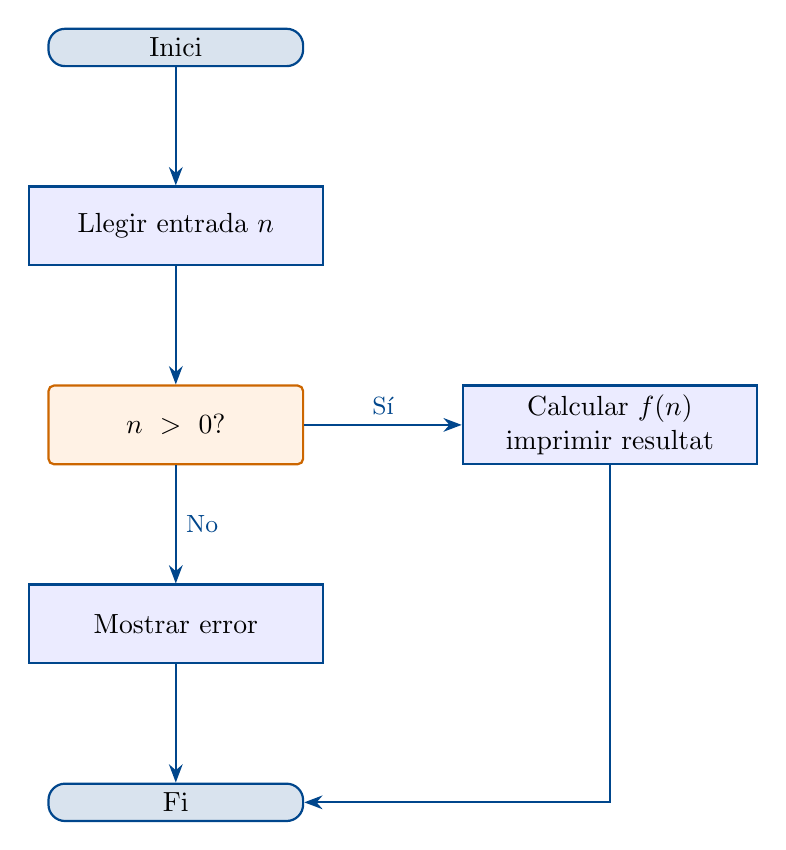
\begin{tikzpicture}[
  node distance=1.5cm and 2cm,
  start/.style={rectangle, rounded corners=6pt, draw=myblue, fill=myblue!15,
                text width=3cm, align=center, thick},
  process/.style={rectangle, draw=myblue, fill=blue!8,
                  text width=3.5cm, align=center, minimum height=1cm, thick},
  decision/.style={rectangle, rounded corners=2pt, draw=orange!80!black, fill=orange!10,
                   text width=3cm, align=center,
                   minimum height=1cm, thick},
  arrow/.style={-Stealth, thick, myblue}
]
  \node[start]    (ini)  {Inici};
  \node[process, below=of ini]  (inp)  {Llegir entrada $n$};
  \node[decision, below=of inp] (dec)  {$n > 0$?};
  \node[process, right=of dec]  (pro)  {Calcular $f(n)$\\imprimir resultat};
  \node[process, below=of dec]  (err)  {Mostrar error};
  \node[start, below=of err]    (fi)   {Fi};

  \draw[arrow] (ini) -- (inp);
  \draw[arrow] (inp) -- (dec);
  \draw[arrow] (dec) -- node[above]{\small Sí} (pro);
  \draw[arrow] (dec) -- node[right]{\small No} (err);
  \draw[arrow] (pro) |- (fi);
  \draw[arrow] (err) -- (fi);
\end{tikzpicture}
\caption{Diagrama de flux d'un algorisme de validació}
\label{fig:flux}
\end{figure}

\subsection{Gràfic de funcions (pgfplots)}

\begin{figure}[H]
\centering
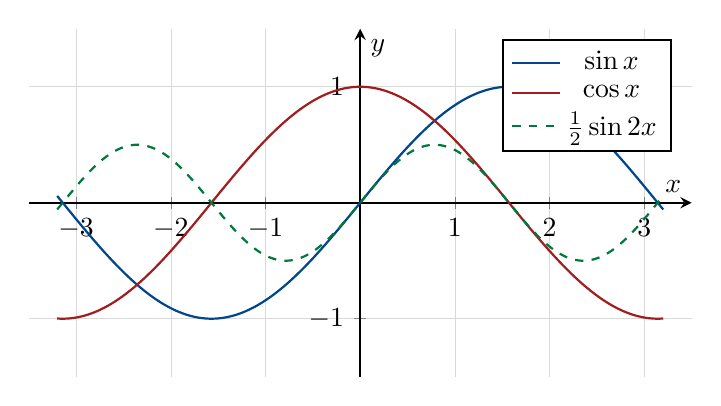
\begin{tikzpicture}
\begin{axis}[
  width=10cm, height=6cm,
  xlabel={$x$}, ylabel={$y$},
  legend pos=north east,
  grid=both, grid style={line width=0.2pt, gray!30},
  axis lines=center,
  xmin=-3.5, xmax=3.5,
  ymin=-1.5, ymax=1.5,
  domain=-3.2:3.2, samples=200,
  thick
]
  \addplot[myblue,  thick] {sin(deg(x))};  \addlegendentry{$\sin x$}
  \addplot[myred,   thick] {cos(deg(x))};  \addlegendentry{$\cos x$}
  \addplot[mygreen, thick, dashed] {sin(deg(2*x))/2}; \addlegendentry{$\frac{1}{2}\sin 2x$}
\end{axis}
\end{tikzpicture}
\caption{Gràfic de funcions trigonomètriques amb \texttt{pgfplots}}
\label{fig:trig}
\end{figure}

\subsection{Diagrama de barres (pgfplots)}

\begin{figure}[H]
\centering
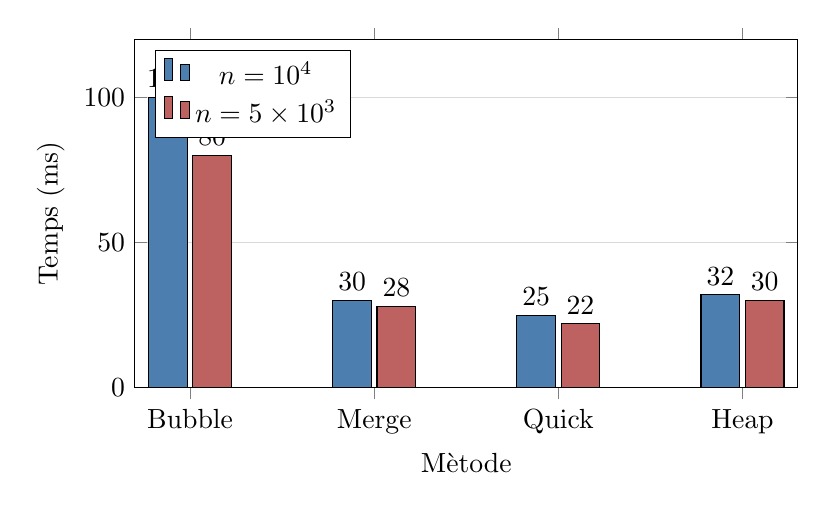
\begin{tikzpicture}
\begin{axis}[
  ybar, width=10cm, height=6cm,
  bar width=14pt,
  xlabel={Mètode}, ylabel={Temps (ms)},
  xtick=data,
  symbolic x coords={Bubble, Merge, Quick, Heap},
  nodes near coords, nodes near coords align={vertical},
  ymin=0, ymax=120,
  ymajorgrids=true, grid style={gray!30},
  legend pos=north west
]
  \addplot[fill=myblue!70]  coordinates {(Bubble,100) (Merge,30) (Quick,25) (Heap,32)};
  \addplot[fill=myred!70]   coordinates {(Bubble,80)  (Merge,28) (Quick,22) (Heap,30)};
  \legend{$n=10^4$, $n=5\times10^3$}
\end{axis}
\end{tikzpicture}
\caption{Comparativa de temps d'execució d'algoritmes d'ordenació}
\label{fig:barres}
\end{figure}


% ═════════════════════════════════════════════
\section{Codi Font i Pseudocodi}
% ═════════════════════════════════════════════

\subsection{Python (listings)}

\begin{lstlisting}[style=python, caption={Cerca binària en Python}, label=cod:binsearch]
def cerca_binaria(llista, objectiu):
    """Retorna l'índex de l'objectiu o -1 si no existeix."""
    esquerra, dreta = 0, len(llista) - 1
    while esquerra <= dreta:
        mig = (esquerra + dreta) // 2
        if llista[mig] == objectiu:
            return mig
        elif llista[mig] < objectiu:
            esquerra = mig + 1
        else:
            dreta = mig - 1
    return -1

# Exemple d'ús
dades = [2, 5, 8, 12, 16, 23, 38, 56, 72, 91]
print(cerca_binaria(dades, 23))  # Resultat: 5
\end{lstlisting}

\subsection{C (listings)}

\begin{lstlisting}[style=c, caption={Factorial recursiu en C}, label=cod:factorial]
#include <stdio.h>

long long factorial(int n) {
    if (n <= 1) return 1;
    return n * factorial(n - 1);
}

int main() {
    for (int i = 0; i <= 10; i++) {
        printf("%d! = %lld\n", i, factorial(i));
    }
    return 0;
}
\end{lstlisting}

\subsection{Pseudocodi (algorithm + algpseudocode)}

\lstdefinestyle{pseudo}{
    mathescape=true,
    basicstyle=\ttfamily\small,
    backgroundcolor=\color{codebg},
    frame=single, rulecolor=\color{codeframe},
    numbers=left, numberstyle=\tiny\color{gray}, numbersep=8pt,
    keywordstyle=\bfseries,
    morekeywords={while, for, if, else, return, end, do},
    showstringspaces=false,
    breaklines=true
}

\begin{tcolorbox}[title=Algorisme 1: Dijkstra, colback=gray!5,
    colframe=myblue, fonttitle=\bfseries, label=alg:dijkstra]
\textbf{Entrada:} Graf $G=(V,E)$ amb pesos $w \geq 0$, node origen $s$\\
\textbf{Sortida:} Distàncies mínimes $d[v]$ per a tot $v \in V$
\begin{lstlisting}[style=pseudo]
$d[s] \gets 0$;  $d[v] \gets \infty$ per a tot $v \neq s$
$Q \gets V$                        // Cua de prioritat
while $Q \neq \emptyset$ do
    $u \gets$ node de $Q$ amb $d[u]$ minim
    eliminar $u$ de $Q$
    for cada vei $v$ de $u$ do
        if $d[u] + w(u,v) < d[v]$ then
            $d[v] \gets d[u] + w(u,v)$
        end if
    end for
end while
return $d$
\end{lstlisting}
\end{tcolorbox}


% ═════════════════════════════════════════════
\section{Química i Física}
% ═════════════════════════════════════════════

\subsection{Fórmules químiques}

Molècules comunes:
H\textsubscript{2}O, \quad CO\textsubscript{2}, \quad NaCl, \quad
C\textsubscript{6}H\textsubscript{12}O\textsubscript{6}, \quad H\textsubscript{2}SO\textsubscript{4}.

Reaccions (amb mode matemàtic per als símbols):
\[
2\,\mathrm{H_2} + \mathrm{O_2} \longrightarrow 2\,\mathrm{H_2O}
\]
\[
\mathrm{CH_4} + 2\,\mathrm{O_2} \longrightarrow \mathrm{CO_2} + 2\,\mathrm{H_2O}
\]

\subsection{Lleis físiques amb unitats}

\textbf{Llei de Newton:} $\vec{F} = m\vec{a}$, on $m = 5\ \text{kg}$ i $a = 9{,}81\ \text{m/s}^2$.

\textbf{Energia cinètica:} $E_c = \dfrac{1}{2}mv^2$

\textbf{Equació d'ona:} $\dfrac{\partial^2 u}{\partial t^2} = c^2 \dfrac{\partial^2 u}{\partial x^2}$

\textbf{Equació de Schrödinger:} $i\hbar\dfrac{\partial}{\partial t}\Psi = \hat{H}\Psi$

\textbf{Equacions de Maxwell:}
\begin{align}
  \nabla \cdot \vec{E} &= \frac{\rho}{\varepsilon_0} \\
  \nabla \cdot \vec{B} &= 0 \\
  \nabla \times \vec{E} &= -\frac{\partial \vec{B}}{\partial t} \\
  \nabla \times \vec{B} &= \mu_0\vec{J} + \mu_0\varepsilon_0\frac{\partial \vec{E}}{\partial t}
\end{align}


% ═════════════════════════════════════════════
\section{Referències i Bibliografia}
% ═════════════════════════════════════════════

\subsection{Referències creuades}

Al document podem fer referència a:
\begin{itemize}
  \item L'equació~\eqref{eq:quadrat} de la secció anterior.
  \item La Taula~\ref{tab:complexitat} de la secció de taules.
  \item La Figura~\ref{fig:trig} amb el gràfic de pgfplots.
  \item El Codi~\ref{cod:binsearch} amb la cerca binària.
  \item El pseudocodi de Dijkstra a la secció de Codi Font.
\end{itemize}

\subsection{Hipervínculs}

\begin{itemize}
  \item Documentació oficial de LaTeX: \url{https://www.latex-project.org}
  \item Text amb hipervíncle ocult: \href{https://ctan.org}{CTAN -- repositori de paquets LaTeX}
  \item Enviar correu: \href{mailto:correo@exemple.com}{correo@exemple.com}
\end{itemize}

\subsection{Citacions bibliogràfiques}

Per citar referències useu \texttt{\textbackslash cite\{clau\}}.
Exemple: la transformada de Fourier es descriu a \cite{oppenheim1999}.

% ─── Llista de referències ───────────────────
\begin{thebibliography}{9}

\bibitem{oppenheim1999}
  A.V. Oppenheim, R.W. Schafer,
  \textit{Discrete-Time Signal Processing}, 2a ed.
  Prentice Hall, 1999.

\bibitem{knuth1997}
  D.E. Knuth,
  \textit{The Art of Computer Programming}, vol.~1--4.
  Addison-Wesley, 1997.

\bibitem{cormen2022}
  T.H. Cormen, C.E. Leiserson, R.L. Rivest, C. Stein,
  \textit{Introduction to Algorithms}, 4a ed.
  MIT Press, 2022.

\end{thebibliography}


% ═════════════════════════════════════════════
\section{Conclusions}
% ═════════════════════════════════════════════

En aquesta plantilla s'han vist els elements essencials de LaTeX per a pràctiques
de qualsevol àrea:

\begin{enumerate}
  \item \textbf{Text i estructura:} format, mides, alineació, llistes, caixes de colors.
  \item \textbf{Matemàtiques:} símbols, lletres gregues, límits, integrals, matrius,
        equacions alineades, teoremes i proves.
  \item \textbf{Física i química:} unitats SI, fórmules químiques, equacions vectorials.
  \item \textbf{Taules:} bàsiques, professionals, multi-fila/columna, dades numèriques.
  \item \textbf{Figures:} imatges, subfigures, diagrames TikZ, gràfics pgfplots.
  \item \textbf{Codi:} Python, C amb ressaltat de sintaxi, pseudocodi estructurat.
  \item \textbf{Referències:} creuades, hipervínculs i bibliografia.
\end{enumerate}


% ═════════════════════════════════════════════
\appendix
\section{Apèndix: Taula de símbols}
% ═════════════════════════════════════════════

\begin{table}[H]
\centering
\begin{tabular}{cll}
  \toprule
  \textbf{Símbol} & \textbf{Comanda LaTeX} & \textbf{Significat} \\
  \midrule
  $\forall$          & \texttt{\textbackslash forall}   & Per a tot \\
  $\exists$          & \texttt{\textbackslash exists}   & Existeix \\
  $\in$              & \texttt{\textbackslash in}       & Pertany \\
  $\subseteq$        & \texttt{\textbackslash subseteq} & Contingut o igual \\
  $\Rightarrow$      & \texttt{\textbackslash Rightarrow} & Implica \\
  $\Leftrightarrow$  & \texttt{\textbackslash Leftrightarrow} & Si i només si \\
  $\nabla$           & \texttt{\textbackslash nabla}   & Gradient/nabla \\
  $\partial$         & \texttt{\textbackslash partial} & Derivada parcial \\
  $\infty$           & \texttt{\textbackslash infty}   & Infinit \\
  $\cancel{x}$       & \texttt{\textbackslash cancel\{x\}} & Cancel·lat \\
  \bottomrule
\end{tabular}
\caption{Símbols matemàtics freqüents}
\end{table}


\end{document}